\documentclass[tikz,border=5mm]{standalone}
\usepackage{amsmath}
\begin{document}
	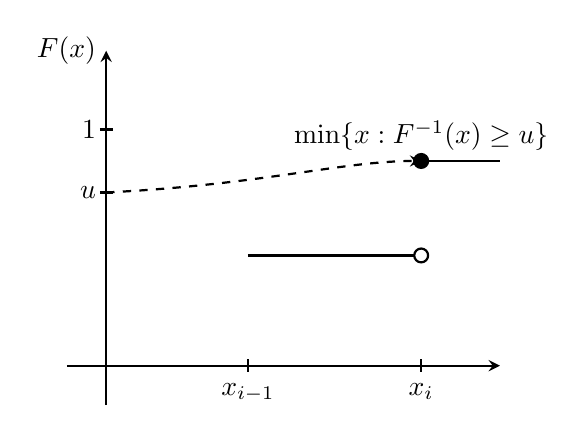
\begin{tikzpicture}[>=stealth, thick]
		
		% Axes
		\draw[->] (-0.5,0) -- (5,0) node[below left] {};
		\draw[->] (0,-0.5) -- (0,4) node[left] {$F(x)$};
		
		% y-axis label M
		\node[left] at (0,2.2) {$u$};
		\draw (-0.08,2.2) -- (0.08,2.2); % tick mark on y-axis
		
		% y-axis label 1
		\node[left] at (0,3) {1};
		\draw (-0.08,3) -- (0.08,3); % tick mark on y-axis

		% dashed arrow from y-axis level $u$ to the jump point
		\draw[dashed,->] (0,2.2) .. controls (2,2.3) and (3,2.6) .. (4,2.6);
		
		% Upper branch: filled circle at (4, 2.6), solid segment extending right
		\node[above] at (4,2.6) {$\min\{x:F^{-1}(x) \ge u\}$};
		\filldraw (4,2.6) circle (2.5pt);
		\draw (4,2.6) -- (5,2.6);
		
		% Lower branch: solid segment ending in open circle at x_i
		\draw (1.8,1.4) -- (4,1.4);
		\draw[fill=white] (4,1.4) circle (2.5pt);
		
		% x-axis ticks
		\draw (1.8,0.08) -- (1.8,-0.08);
		\node[below] at (1.8,-0.1) {$x_{i-1}$};
		
		\draw (4,0.08) -- (4,-0.08);
		\node[below] at (4,-0.1) {$x_i$};
		
		
	\end{tikzpicture}
\end{document}